\chapter{Mathematical modeling}

\section{Understanding mathematical modeling}

Modeling is one of the ways to solve problems that appear in the real world [4]. In many cases we cannot afford finding the right solutions by experimenting   with real objects:  building, destroying, making changes may be too expensive, dangerous, or just impossible. If this is so, we leave the real world and go up to the world of models, see the Figure 1. We build a model of a real system: its representation in a modeling language. This process assumes abstraction: we throw away the details that are irrelevant to the problem we are trying to solve and keep what we think is important. The model is always less complex than the real system. Having built the model ( or sometimes  even while building the model ) , we  start to explore and understand the structure and behavior of the original system, test how the system will behave under various conditions, play  and compare different scenarios, optimize.  When we find the solution we are looking for, we map that solution back to the real world.

\begin{figure}
   \centering
	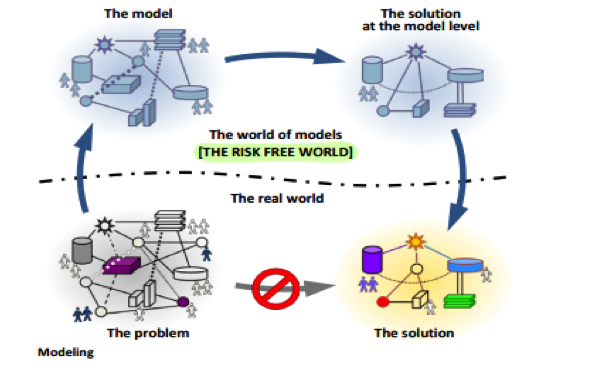
\includegraphics[width=0.9\textwidth]{img/modeling}
	\caption[Clear]{Mathematical modeling benefits visualization}
\end{figure}

Models are used and successfully applied in different areas starting from logistics to health care systems. Types of modeling include conceptual modeling, analytical modeling and simulation modeling.

\section{Types of epidemic models}

Modeling in the field of epidemiology has been of interest long ago (application of mathematical methods in the study of epidemic began in the middle of the XVII century) [7].Since that time, the methods of infectious diseases modeling gradually improved, the different variants of models appeared, reflecting the characteristics of the studied processes [7]. However, it cannot be concluded that the problem is solved. The earliest mathematical epidemic model was constructed by Daniel Bernoulli in 1766 [8]. The results showed that the universal inoculation against smallpox could increase the life expectancy [8]. But the real progress in modeling was made in XX century when Hammer(1906), Ross(1911, 1916) and A. G. McKendrick and W.O. Kermack (1927) formulated a simple deterministic model based on the moving matters and homogeneity of crossing [8]. Ross, in 1910, made a great impact on the improvement of epidemic modeling when he built the malaria spreading model which was based on the concept of reproductive number. However, it was then understood that the process of epidemic spreading is not trivial and simple because it depends on the numerous factors, parameters and variables. Analysis of such kind of parameterized modeling was difficult to achieve until the appearance of computers. Besides, the infectious diseases had been reducing during the 2nd half of XX century and thus there was no need in epidemic modeling. With the appearance of computers, the situation changed and special software packages for modeling were given rise.

In fact, the infection spreading tendency can be modeled by 2 approaches: extrapolation models and dynamic models [8].

\subsection{Extrapolation models}

Extrapolation itself means relying on a prior knowledge of the process that created the existing data points [6]. So, the morbidity data of the past is gathered first. Then, it’s assumed that the further behavior of the process will be the same as in the past. If there is wave like rise in the disease spreading, the frequency of such rise is defined and the time of next rise can be predicted. The most popular method of decomposing is Fourier series which can describe any periodic process [6]. However, Fourier series considers that parameters change constantly when in fact, variations occur in random way. This problem can be solved by segmenting the population into different groups with different characteristics and separately analyzing each of them, and then defining total rates of subgroups. For example, old people get flu more often than others, so, this group’s morbidity rate will increase the total morbidity rate of population. As we divided the population into segments, now we must identify the key parameters of morbidity and determine their impact on the morbidity rate. This can be done by regression equations as a form of the functions that describe the changes of process to be dependent on not only time but on those factors as well [6].However, making the regression analysis will be too complicated in this case as we must take into account different variables for different classes of population. The infection is transmitted from human to human but humans cannot be considered as uniform objects because each person is a unique individual who has own characteristics such as age, status, etc. So, there is a sequential logic in disease spreading. It means that the value at one moment depends on the value of previous moment. Also, the parameters of humans can correlate between each other and overlap. It is known as autocorrelation. Thus, regression cannot be applied in such conditions. As the infection spreading has a wave like character, there is a need in non-linear static models [6].However, there are problems with non-linearity. First, non-linear models are considerably difficult to describe and adjust than linear ones. Second, more historical data are required. So, we see that extrapolation doesn’t work with new forms of disease as there is no past data and information to use. And also, extrapolation considers that all factors that lead to morbidity rate changes are constant whereas the epidemic has a tendency to change and vary as population changes. Usually, for extrapolation modeling, spreadsheet (Excel) is used.

\subsection{Dynamic Models}

Dynamic models describe the disease spreading process among population using mathematical laws [6]. Dynamic models are based on the concept of randomization and probability theory. Also, every possibility or change in the spreading is considered and taken into account. Dynamic models can be divided into 2 types:

a) Stochastic models – are based on the randomization. They incorporate randomness into the model i.e. includes the points that would give random results each time you pass them during the model implementation. They attempt to model the process analogical to real life [6]. So, relationship between separate objects is modeled separately. For example, the contacts between people in the population are modeled and if one person is infected, the second person can be infected with particular probability. This probability is usually done by probability distribution functions. So, stochastic models are used to estimate the probabilistic quantities for the outcome events, such as the probability distribution of extinction time, the probability distribution of final epidemic size, and the associate mean and so on. Stochastic models can be easily applied in the population with limited size as every person’s relation is modeled.

b) Deterministic compartmental models–In deterministic model no randomness is involved. Outcomes are precisely defined through constant variables. In the deterministic compartmental model, we consider that the population is divided into different subgroups or compartments, which represent a specific stage of the epidemic. The transition rates from one class to another are mathematically expressed as derivatives, hence the model is formulated using differential equations. While building such models, it must be assumed that the population size in a compartment is differentiable with respect to time and that the epidemic process is deterministic. In other words, the changes in population of a compartment can be calculated using only the history used to develop the model [9].

\section{Existing traditional models of epidemics spreading}

The most popular method of modeling the epidemics is based on the use of differential equations. In these models, the dynamics of the spread of the disease is described by a system of differential equations, where the numbers of sick and healthy people of the modeled area serve as the variable states [9]. The solution of such system of equations gives the level of infection rates at each moment of the model time. In order to make model, parameters must be defined. In the epidemic models, the following variables are used:

\begin{itemize}
\item $R$: Removed with Immunity
\item $S$: Susceptibles
\item $\beta$: Contact Rate
\item $E$: Exposed Individuals in the Latent Period
\item $N$: Total Population
\item $1/\gamma$: Average Infectious Period
\item $\mu$: Average Death Rate
\item $I$: Infectives
\item $1/\epsilon$: Average Latent Period
\item $f$: Average Loss of Immunity Rate of Recovered Individuals
\item $\delta$: Average Temporary Immunity Period
\item $R_0$: Basic Reproduction Number
\item $B$: Average Birth Rate
\end{itemize}

Epidemiological modeling and its types with different formulas is discussed further in the next section.
